\documentclass[main.tex]{subfiles}

\begin{document}

\textcolor{red}{Лекция 26.03.2022.}

\section{Пороупругость}

Самый важный геомеханический раздел в контексте разработки месторождений.

Вспомним полученное ранее замыкающее соотношение на тензор \textbf{полных} напряжений \eqref{StressTens} (пусть нет начальных напряжений): 
\beq\label{PoroElast1}
T_{ij}=\overbrace{L_{ijkl}\varepsilon_{kl}}^{\substack{\text{эффективные}\\\text{напряжения}}}-\underbrace{\alpha_{ij}\left(p-p_0\right)}_{\substack{\text{пороупругая}\\\text{часть}}}-\overbrace{\alpha_{kl}^{\theta}L_{ijkl}\left(\theta-\theta_0\right)}^{\substack{\text{термические}\\\text{напряжения}}}
\eeq

Вспомним полученное ранее замыкающее соотношение на пористость \eqref{PhiConsRel}:
\beq\label{PoroElast2}
\varphi-\varphi_0=\alpha_{ijkl}\varepsilon_{ij}+\frac{p-p_0}{N}+\alpha_\theta^\varphi\left(\theta-\theta_0\right)
\eeq

Сейчас положительными считаем растягивающие напряжения.

\textbf{Важно!} Эффективные напряжения не равны скелетным напряжениям.

Выпишем связи между полными/скелетными деформациями/напряжениями.

Связь между полной деформацией и деформацией скелета (с точки зрения механики сплошных сред это определение скелетной деформации):
\beq\label{PoroElastRelationship1}
\varepsilon_{ij}=\left(1-\varphi\right)\varepsilon_{ij}^s+\left(\varphi-\varphi_0\right)\delta_{ij}
\eeq

Связь между полным напряжением и напряжением скелета (получали ранее):
\beq\label{PoroElastRelationship2}
T_{ij}=\left(1-\varphi\right)\sigma_{ij}^s-\varphi p\delta_{ij}
\eeq


\subsection{Изотропный случай}
Перепишем равенство \eqref{PoroElast1} в изотропном случае:
\beq\label{IsotropicPoroElast1}
T_{ij}=\overbrace{K\varepsilon_{kk}\delta_{ij}+2G\left(\varepsilon_{ij}-\frac{1}{3}\varepsilon_{kk}\delta_{ij}\right)}^{\text{эффективные напряжения}}-\underbrace{\alpha \left(p-p_0\right)\delta_{ij}}_{\substack{\text{пороупругая}\\\text{часть}}}-\overbrace{3\alpha^{\theta}K\left(\theta-\theta_0\right)\delta_{ij}}^{\text{термические напряжения}}
\eeq

Перепишем равенство \eqref{PoroElast2} в изотропном случае:
\beq\label{IsotropicPoroElast2}
\varphi-\varphi_0=\alpha\varepsilon_{kk}+\frac{p-p_0}{N}+\alpha_\theta^\varphi\left(\theta-\theta_0\right)
\eeq

Закон Гука для материала скелета в изотропном случае:
\beq\label{SkeletGook}
\sigma_{ij}^s=K_s\varepsilon_{kk}^s\delta_{ij}+2G\left(\varepsilon_{ij}^s-\frac{1}{3}\delta_{ij}\varepsilon_{kk}^s\right)
\eeq

Далее \textbf{температура фиксирована} ($\theta=\theta_0$).

Введём обозначения для следов соответствующих тензоров
\beq
\varepsilon^s=\varepsilon_{kk}^s, \varepsilon=\varepsilon_{kk}, \sigma=T_{kk}, \sigma^s=\sigma_{kk}^s
\eeq
тогда из равенства \eqref{IsotropicPoroElast1}, применяя след к обеим частям, получаем:
\beq\label{TraceIsotropicPoroElast1}
\sigma=K\varepsilon-\alpha\left(p-p_0\right)
\eeq
и из равенства \eqref{IsotropicPoroElast2}, применяя след к обеим частям, получаем:
\beq\label{TraceIsotropicPoroElast2}
\varphi-\varphi_0=\alpha\varepsilon+\frac{p-p_0}{N},
\eeq
и из равенства \eqref{SkeletGook}, применяя след к обеим частям, получаем:
\beq\label{TraceSkeletGook}
\sigma^s=K_s\varepsilon^s
\eeq
и из равенства \eqref{PoroElastRelationship1}, применяя след к обеим частям, получаем:
\beq\label{TracePoroElastRelationship1}
\varepsilon=\left(1-\varphi\right)\varepsilon^s+\left(\varphi-\varphi_0\right),
\eeq
и из равенства \eqref{PoroElastRelationship2}, применяя след к обеим частям, получаем:
\beq\label{TracePoroElastRelationship2}
\sigma=\left(1-\varphi\right)\sigma^s-\varphi p
\eeq

Далее будем получать формулы для константы Био и модуля Био (их зависимость от пористости и характеристик материала).
 
\subsubsection{Константа Био}
Рассмотрим образец пористого материала и будем со всех сторон действовать на него сжимающей нагрузкой $d\sigma$ и изнутри через поры будем действовать давлением $dp$. Другими словами, за счёт сжатия прессом сверху и обжатия образца с боков можем сделать равномерное напряжение. Дополнительно через пресс герметично подаём жидкость, увеличивая тем самым давление.

Пусть $dp=-d\sigma$, тогда имеем \textbf{всестороннее сжатие скелета} (фактически со всех сторон образца обжимаем его напряжением $d\sigma$ и изнутри на границах пор и скелета тоже обжимаем напряжением $d\sigma$).

Формально из \eqref{TracePoroElastRelationship2}:
\beq\label{SkeletonCompression}
d\sigma=\left(1-\varphi\right)d\sigma^s-\varphi dp\xRightarrow{dp\,=\,-d\sigma} d\sigma\left(1-\varphi\right)=\left(1-\varphi\right)d\sigma^s\Rightarrow d\sigma=d\sigma^s
\eeq
(действительно, получили всестороннее сжатие скелета).

\begin{figure}[h]
\centering
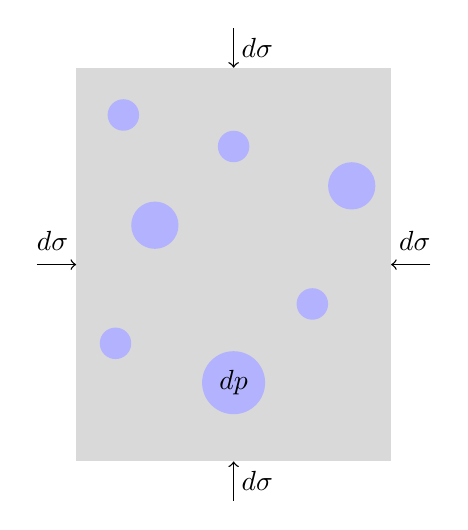
\begin{tikzpicture}[line width=0.5]
\fill[gray!30!white] (1,1) rectangle (5,6);
%\draw[gray] (1,1) -- (5,1) -- (5,6) -- (1,6) -- (1,1);
\fill[blue!30!white] (3,2) circle (0.4cm);
\node at (3,2) {$dp$};
\fill[blue!30!white] (4,3) circle (0.2cm);
\fill[blue!30!white] (2,4) circle (0.3cm);
\fill[blue!30!white] (3,5) circle (0.2cm);
\fill[blue!30!white] (1.6,5.4) circle (0.2cm);
\fill[blue!30!white] (4.5,4.5) circle (0.3cm);
\fill[blue!30!white] (1.5,2.5) circle (0.2cm);
\draw [->] (5.5,3.5) -- (5,3.5);
\node at (5.3,3.8) {$d\sigma$};
\draw [->] (3,0.5) -- (3,1);
\node at (3.3,0.75) {$d\sigma$};
\draw [->] (0.5,3.5) -- (1,3.5);
\node at (0.7,3.8) {$d\sigma$};
\draw [->] (3,6.5) -- (3,6);
\node at (3.3,6.25) {$d\sigma$};
\end{tikzpicture}
\caption{Эксперимент на всестороннее сжатие скелета}
\end{figure}

Из закона Гука для материала скелета \eqref{TraceSkeletGook}:
\beq\label{ExperimentGook}
\varepsilon^s=\frac{d\sigma^s}{K_s}
\eeq

С другой стороны, есть уравнение пороупругости \eqref{TraceIsotropicPoroElast1}:
\beq\label{ExperimentPoroElast1}
d\sigma=K\varepsilon-\alpha dp\xRightarrow{dp\,=\,-d\sigma}d\sigma\left(1-\alpha\right)=K\varepsilon
\eeq

Тогда, учитывая равенство \eqref{SkeletonCompression} (оно верно в рассматриваемом эксперименте), из \eqref{ExperimentGook} и \eqref{ExperimentPoroElast1} получаем
\beq\label{SomeEquality}
K_s\varepsilon^s=\frac{K\varepsilon}{1-\alpha}
\eeq

Предположим, что $K_s=K_f$, тогда $\varepsilon=\varepsilon^s$ (так как при равенстве $K_s=K_f$ образец деформируется как единое целое) и из \eqref{SomeEquality}
\beq\label{ConstBioFinal}
\alpha=1-\frac{K}{K_s},
\eeq
где $K$ -- модуль всестороннего сжатия (сжимаемость) структуры образца и $K_s$ -- сжимаемость скелета.

Но из определения \eqref{3} мы знаем, что $\alpha$ это характеристика скелета и его структуры, то есть $\alpha$ не зависит от свойств флюида. Поэтому равенство \eqref{ConstBioFinal} верно всегда (и при $K_s\neq K_f$).

Таким образом, получили окончательное выражение \eqref{ConstBioFinal} на константу Био $\alpha$.

У очень пористых материалов $\alpha\approx1$, так как у пористых материалов $K\ll K_s$.

\subsubsection{Модуль Био}

Продолжаем рассматривать эксперимент на всестороннее сжатие скелета, в котором $dp=-d\sigma$, тогда выражение \eqref{TraceIsotropicPoroElast2} перепишется для этого эксперимента в следующем виде:
\beq
\varphi-\varphi_0=\alpha\varepsilon+\frac{dp}{N}=\alpha\varepsilon-\frac{d\sigma}{N}
\eeq

С другой стороны, из \eqref{TracePoroElastRelationship1}:
\beq
\varphi-\varphi_0=\varepsilon-\varepsilon^s\left(1-\varphi\right)
\eeq

Приравнивая 2 последних равенства, получаем
\beq
\varepsilon-\varepsilon^s\left(1-\varphi\right)=\alpha\varepsilon-\frac{d\sigma}{N}
\eeq

учитывая, что в рассматриваемом эксперименте $\displaystyle{}\varepsilon=\varepsilon^s=\frac{d\sigma^s}{K_s}=\frac{d\sigma}{K_s}$, из последнего равенства получаем
\beq
\frac{1-\alpha}{K_s}+\frac{1}{N}-\frac{1-\varphi}{K_s}=0
\eeq
и окончательное выражение для модуля Био:
\beq
\frac{1}{N}=\frac{\alpha-\varphi}{K_s}
\eeq

Видим, что если $\alpha=\varphi$, то модуля Био не существует и скелетные напряжения не отличаются от эффективных.

\subsection{Задача для закрепления}

В общем случае скелетные напряжения $\sigma_{ij}^s$ не совпадают с эффективными напряжениями $L_{ijkl}\varepsilon_{kl}$. Скелетные напряжения используются только в теоретических выводах (не фигурируют в практических задачах).

Рассмотрим пористый материал.
\begin{figure}[h]
\centering
\begin{tikzpicture}[line width=0.5]
\fill[orange!30!white] (1,1) rectangle (7,5);
%\draw[gray] (1,1) -- (5,1) -- (5,6) -- (1,6) -- (1,1);
\fill[black!30!white] (3,2) circle (0.4cm);
\node at (3,2) {$p$};
\fill[blue!30!white] (4,3) circle (0.2cm);
\fill[blue!30!white] (2,4) circle (0.3cm);
\fill[blue!30!white] (5,3) circle (0.2cm);
\fill[blue!30!white] (5.4,1.6) circle (0.2cm);
\fill[blue!30!white] (6,4) circle (0.2cm);
\fill[black!40!white] (4.5,4.5) circle (0.3cm);
\fill[blue!30!white] (1.5,2.5) circle (0.2cm);
\node at (8.5,4) {$p=250\text{ атм}$};
\node at (8.5,3) {$\alpha=0.8$};
\node at (8.5,2) {$\varphi=0.2$};
\draw [->] (4,5.5) -- (4,5);
\node at (5.25,5.4) {$T=400\text{ атм}$};
\end{tikzpicture}
\caption{К задаче о скелетных и эффективных напряжениях}
\end{figure}

Найдём скелетные и эффективные напряжения, чтобы почувствовать разницу.

Скелетные напряжения из связи \eqref{PoroElastRelationship2}:
\beq
\sigma_{ij}^s=\frac{T_{ij}-p\varphi\delta_{ij}}{1-\varphi}
\eeq

Эффективные напряжения при постоянной температуре из уравнения пороупругости \eqref{PoroElast1}:
\beq
\sigma_{ij}'=T_{ij}-\alpha_{ij}p
\eeq

Подставляем исходные данные задачи в выражение для скелетных напряжений:
\beq
\sigma^s=\frac{400-0.2\cdot250}{0.8}=437.5\text{ (атм)}
\eeq
и для эффективных напряжений:
\beq
\sigma'=400-0.8\cdot250=200\text{ (атм)}
\eeq

Скелетные напряжения действуют прямо в скелете. Они существуют в реальности, но для практического решения задач не подходят, так как мы не можем измерить деформацию скелетного материала, а можем только измерить деформацию керна в целом.

Эффективные напряжения вводятся для удобства расчётов: вычленяем их из полных напряжений $T_{ij}$, чтобы посчитать деформацию образца керна. Эффективные напряжения не соответствуют каким либо реальным напряжениям, имеющимся в породе.

\subsection{2 эксперимента над керном для определения пороупругих констант}

\begin{figure}[h]
\centering
\begin{tikzpicture}[line width=0.5]
\draw (0,0) rectangle (6,7);
\fill[orange!30!white] (1,1) rectangle (5,6);
\fill[blue!30!white] (4.65,1.7) circle (0.3cm);
\draw (4.9,1.5) -- (7.5,1.5) -- (7.5,3);
\draw (4.9,1.7) -- (7.3,1.7) -- (7.3,3);
\node at (8.7,3.4) {$1\text{ атм -- давление снаружи}$};
\fill[blue!30!white] (4.8,1.51) rectangle (7.32,1.69);
\fill[blue!30!white] (7.31,1.51) rectangle (7.49,2);
%\draw[gray] (1,1) -- (5,1) -- (5,6) -- (1,6) -- (1,1);
\fill[blue!30!white] (3,2) circle (0.4cm);
\node at (3,2) {$dp$};
\fill[black!40!white] (4,3) circle (0.2cm);
\fill[blue!30!white] (2,4) circle (0.3cm);
\fill[blue!30!white] (3,5) circle (0.2cm);
\fill[black!40!white] (1.6,5.4) circle (0.2cm);
\fill[blue!30!white] (4.5,4.5) circle (0.3cm);
\fill[blue!30!white] (1.5,2.5) circle (0.2cm);
\draw [->] (5.5,3.5) -- (5,3.5);
\node at (5.3,3.8) {$d\sigma$};
\draw [->] (3,0.5) -- (3,1);
\node at (3.3,0.75) {$d\sigma$};
\draw [->] (0.5,3.5) -- (1,3.5);
\node at (0.7,3.8) {$d\sigma$};
\draw [->] (3,6.5) -- (3,6);
\node at (3.3,6.25) {$d\sigma$};
\node at (1,6.6) {$dP=d\sigma$};
\draw[dashed] (4.5,5.5) -- (6.5,6);
\node at (7.5,6.2) {$\substack{\text{Керн в эластичной}\\\text{оболочке}}$};
\draw[dashed] (6,4) -- (7,4.5);
\node at (8.5,4.9) {$\substack{\text{Герметичная камера}\\\text{(с регулируемым давлением внутри)}}$};

\end{tikzpicture}
\caption{Схема первого эксперимента над керном}
\end{figure}

\section{Решение задач}


\end{document}
